\chapter{Conclusion}

\section{Future Work}

\subsection{Signed Distance Fields}

Pixar has published OpenVDB which helps
work around these concerns, but such compression can be lossy.\cite{OpenVDB}
With the advent of shader pipelines for GPUs, distance fields have become
more popular. Valve has used SDFs with great success for generating smooth
text renders. \cite{Green_2007}
Many algorithms for generating polyhedra from an SDF
exist. The most common are Marching Tetrahedra, Marching Cubes,
and Dual Contours.\cite{Muller_Wehle_1997}\cite{Newman_Yi_2006}\cite{Cook_Hourvitz}

Andreas Bærentzen and Henrik Aanæs published methods on the inverse
problem of converting a mesh to a signed distance fields.\cite{Baerentzen_Aanaes}
DiFi was introduced in 2004, which demonstrates an algorithm for creating
SDFs on multiple types of geometry \cite{Sud_Otaduy_Manocha_2004}.

Many necessary algorithms in path planning for digital manufacturing tools
fall out of distance fields. For example, offsetting simply becomes
an addition or subtraction over the SDF. Computing the medial axis becomes
a scan for inflection points. Many path planners need to simplify polygon
representations as to not generate move less than the resolution of the machine.
Assuming the machine uses a Cartesian system, a SDF can correspond perfectly
to the lowest available resolution of the machine.
Likewise as Stereolithographic 3D printers
begin to use digital mirror devices (commonly known as DLP or DMD)
, discrete representations of geometry will become more important in
digital manufacturing.

\subsection{Automatic Differention of Solids}

\begin{lstlisting}
julia> using DualNumbers

julia> f(x) = 2x+1
f (generic function with 1 method)

julia> f(Dual(1,1))
3 + 2du
\end{lstlisting}



\subsection{Ray Tracing and Marching}

\todo{leave this section, would be good to discuss angle-based polyhedra
and or deficits for these ops}

When we look at the natural world we observe the
propogation of light energy. Our eyes recieve this light energy in the form
of photons. The study of ray tracing seeks to mimic such behavior for
computer visualizations and simulations. 

\begin{figure}[h!]
  \centering
    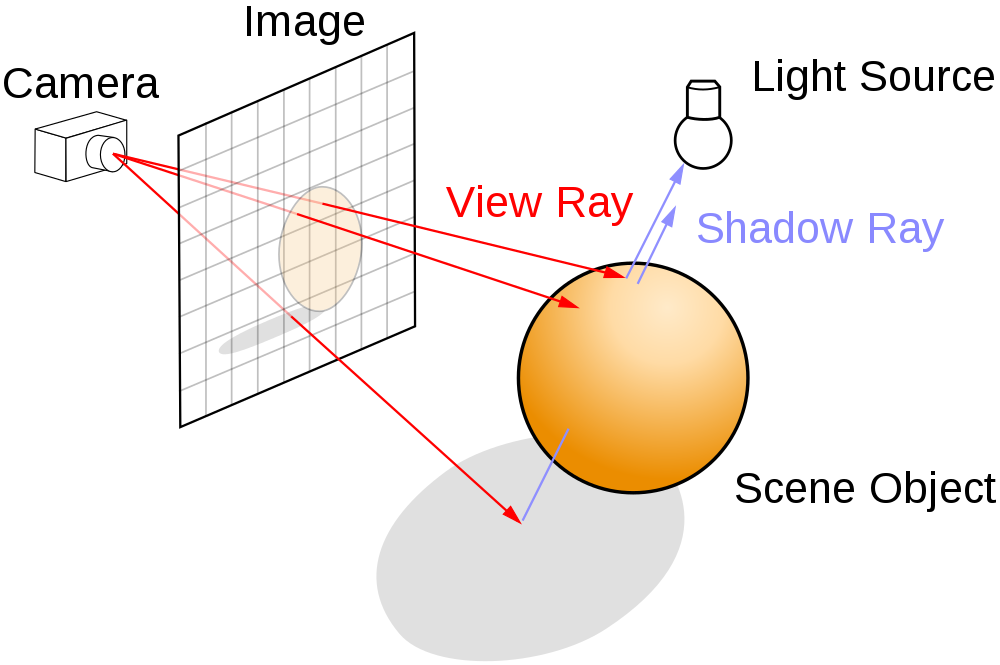
\includegraphics[width=0.75\textwidth]{img/ray_trace_diagram.png}
  \caption{An illustration of a Ray tracing.\protect\footnotemark}
  \label{fig:raytrace}
\end{figure}

\footnotetext{By Henrik (Own work) GFDL or CC BY-SA 4.0-3.0-2.5-2.0-1.0, via Wikimedia Commons}

Íñgo Quílez has done some of the most accessible work on real-time ray tracing.
His technique is called ray marching, and leverages the properties of functional
geometry.\cite{Quilez_2008}

\subsection{Engineering Solid Analysis}



